% Compile with XeLaTeX or LuaLaTeX (Metropolis theme uses system fonts);
% pdfLaTeX also works through the fallback fonts below.
\documentclass[9pt,aspectratio=169]{beamer}

% ================= THEME =================
\usetheme{metropolis}
\metroset{block=fill,progressbar=frametitle,numbering=fraction,sectionpage=none}

% ================= FONTS =================
\usepackage{iftex}
\ifpdftex
  % pdfLaTeX (default Overleaf compiler)
  \usepackage[utf8]{inputenc}
  \usepackage[T1]{fontenc}
  \usepackage{lato}
  \usepackage[scale=0.82]{FiraMono}
\else
  % XeLaTeX / LuaLaTeX
  \usepackage{fontspec}
  \IfFontExistsTF{Lato}{
    \setmainfont{Lato}
    \setsansfont{Lato}
  }{
    \usepackage{lato}
  }
  \IfFontExistsTF{Fira Code}{
    \setmonofont{Fira Code}[Scale=0.82]
  }{
    \usepackage[scale=0.82]{FiraMono}
  }
\fi

% ================= PACKAGES =================
\usepackage{listings}
\usepackage{url}
\usepackage{xcolor}
\usepackage{tikz}
\usetikzlibrary{arrows.meta,positioning,fit,backgrounds,calc}
\usepackage{booktabs}
\usepackage{amsmath}
\usepackage{array}

% ================= COLOR PALETTE =================
\definecolor{primary}{HTML}{0E2A3F}      % deep petrol navy
\definecolor{secondary}{HTML}{1A7A6E}    % teal
\definecolor{accent}{HTML}{E0A32E}       % warm amber
\definecolor{accent2}{HTML}{C1502E}      % terracotta
\definecolor{bgcream}{HTML}{FAF7F0}      % warm off-white background
\definecolor{inkgrey}{HTML}{2B2B2B}

\setbeamercolor{background canvas}{bg=bgcream}
\setbeamercolor{normal text}{fg=primary}
\setbeamercolor{frametitle}{bg=primary,fg=bgcream}
\setbeamercolor{progress bar}{fg=accent,bg=primary!25}
\setbeamercolor{title separator}{fg=accent}
\setbeamercolor{alerted text}{fg=accent2}
\setbeamercolor{example text}{fg=secondary}
\setbeamercolor{block title}{bg=secondary,fg=bgcream}
\setbeamercolor{block body}{bg=secondary!10,fg=primary}
\setbeamercolor{block title alerted}{bg=accent2,fg=bgcream}
\setbeamercolor{block body alerted}{bg=accent2!10,fg=primary}
\setbeamercolor{block title example}{bg=primary!85,fg=bgcream}
\setbeamercolor{block body example}{bg=primary!8,fg=primary}
\setbeamercolor{itemize item}{fg=secondary}
\setbeamercolor{itemize subitem}{fg=accent2}
\setbeamertemplate{itemize item}{\raisebox{0.15ex}{\textbullet}}

% ================= CODE STYLE =================
\definecolor{codebg}{HTML}{F1ECDF}
\definecolor{codekw}{HTML}{0E2A3F}
\definecolor{codecom}{HTML}{8A8A82}
\definecolor{codestr}{HTML}{C1502E}
\lstset{
  basicstyle=\ttfamily\scriptsize,
  keywordstyle=\color{codekw}\bfseries,
  commentstyle=\color{codecom}\itshape,
  stringstyle=\color{codestr},
  backgroundcolor=\color{codebg},
  showstringspaces=false,
  breaklines=true,
  frame=single,
  rulecolor=\color{primary!25},
  xleftmargin=4pt,
  xrightmargin=4pt,
  language=Python,
  columns=fullflexible
}

% ================= TIKZ NODE STYLES (model diagrams) =================
\tikzset{
  layer/.style={draw=primary, thick, rounded corners=2pt, fill=secondary!12,
    minimum height=7mm, align=center, font=\scriptsize, text=primary},
  layerhi/.style={draw=accent2, thick, rounded corners=2pt, fill=accent!25,
    minimum height=7mm, align=center, font=\scriptsize, text=primary},
  tok/.style={draw=primary, thick, rounded corners=1pt, fill=secondary!15,
    minimum width=6mm, minimum height=6mm, font=\tiny, text=primary},
  clstok/.style={draw=accent2, thick, rounded corners=1pt, fill=accent!35,
    minimum width=6mm, minimum height=6mm, font=\tiny, text=primary},
  tree/.style={draw=primary, thick, fill=secondary!12, minimum width=9mm,
    minimum height=6mm, align=center, font=\tiny, text=primary},
  flowarr/.style={-{Stealth[length=2mm]}, thick, primary},
  attn/.style={-, accent2!70, opacity=0.55}
}

\title{MoA Prediction}
\subtitle{Multi-Model Ensemble for Mechanisms-of-Action Classification}
\author{Marco Merlonghi}
\date{\today}

\begin{document}

% ---------------------------------------------------------------
% TITLE
% ---------------------------------------------------------------
\begin{frame}[plain]
  \begin{tikzpicture}[remember picture, overlay]
    \fill[primary] (current page.south west) rectangle (current page.north east);
    \fill[secondary!85] ([xshift=-2cm,yshift=1.4cm]current page.south west) --
      ([xshift=6cm,yshift=1.4cm]current page.south west) --
      ([xshift=2cm,yshift=-1cm]current page.south west) -- cycle;
    \fill[accent] ([xshift=-1cm,yshift=-0.2cm]current page.north east) --
      ([xshift=-7cm,yshift=-0.2cm]current page.north east) --
      ([xshift=-3cm,yshift=1.6cm]current page.north east) -- cycle;
    \node[anchor=west, text=bgcream, font=\Huge\bfseries] at ([xshift=1cm,yshift=1cm]current page.west)
      {MoA Prediction};
    \node[anchor=west, text=accent, font=\Large] at ([xshift=1.05cm,yshift=0.2cm]current page.west)
      {A Multi-Model Ensemble for Mechanism-of-Action Classification};
    \node[anchor=west, text=bgcream!70, font=\small] at ([xshift=1.05cm,yshift=-0.7cm]current page.west)
      {Marco Merlonghi \quad\textbar\quad Project Work in Machine Learning and Data Mining};
  \end{tikzpicture}
\end{frame}

\section{The Challenge}

% ---------------------------------------------------------------
% ABOUT THE COMPETITION
% ---------------------------------------------------------------
\begin{frame}{About the Competition}
  \begin{columns}[T]
    \begin{column}{0.58\textwidth}
      \begin{itemize}
        \item \textbf{Host:} Laboratory for Innovation Science at Harvard (LISH), with the Broad Institute's Connectivity Map (LINCS);
        \item \textbf{Platform:} Kaggle -- \url{https://kaggle.com/c/lish-moa};
        \item \textbf{Timeline:} launched and closed in 2020 (final deadline Nov.\ 30, 2020);
        \item \textbf{Scale:} several thousand teams (see the Kaggle leaderboard page);
        \item \textbf{Data origin:} L1000 assay -- a high-throughput assay measuring how human cell lines respond transcriptionally to a chemical or genetic perturbation.
      \end{itemize}
    \end{column}
    \begin{column}{0.42\textwidth}
      \begin{block}{Why it matters}
        Mapping a compound's gene-expression and cell-viability signature to its mechanism of action accelerates \textbf{drug discovery} and \textbf{repurposing}, replacing slow, costly wet-lab characterisation with a computational first pass.
      \end{block}
    \end{column}
  \end{columns}
\end{frame}

% ---------------------------------------------------------------
% THE PROBLEM AND THE DATA
% ---------------------------------------------------------------
\begin{frame}{The Problem and the Data}
  \begin{columns}[T]
    \begin{column}{0.55\textwidth}
      \begin{itemize}
        \item \textbf{Task:} multi-label classification of \textbf{206 mechanisms of action (MoA)}
        \item \textbf{Input:} 772 gene-expression (\texttt{g-}) and 100 cell-viability (\texttt{c-}) features, plus \texttt{cp\_time} and \texttt{cp\_dose}
        \item \textbf{Size:} $\approx$23.8k training rows, $\approx$22k after removing controls
        \item \textbf{Imbalance:} positives are very rare (mean predicted probability on treated test rows: 0.0037)
        \item \textbf{Metric:} mean multi-label binary log loss, clipped to avoid $\log(0)$
        \item Control rows (\texttt{cp\_type == ctl\_vehicle}) carry \textbf{no MoA}: excluded from training, set to 0 at submission
      \end{itemize}
    \end{column}
    \begin{column}{0.45\textwidth}
      \begin{block}{Why an ensemble?}
        Dense nets and tree models fail differently on rare positives $\Rightarrow$ blending several architectures on different preprocessing variants reduces variance.
      \end{block}
    \end{column}
  \end{columns}
\end{frame}

\section{Pipeline Overview}

% ---------------------------------------------------------------
% PIPELINE AT A GLANCE
% ---------------------------------------------------------------
\begin{frame}{Pipeline at a Glance}
  \centering
  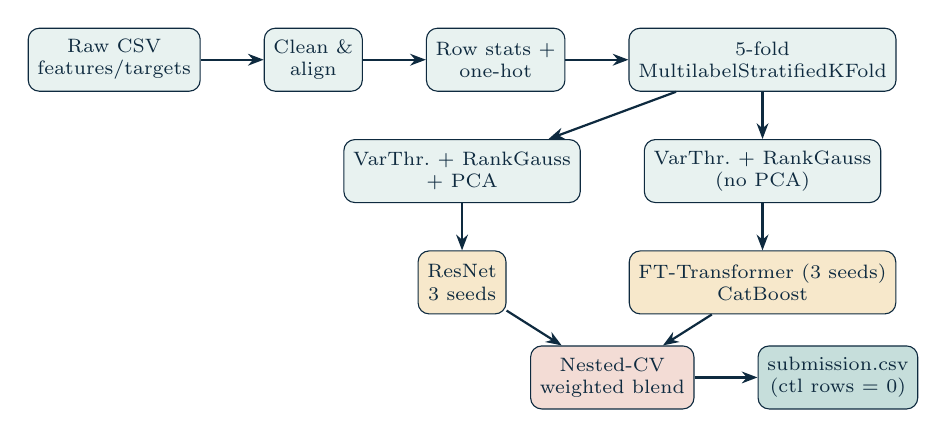
\begin{tikzpicture}[
      node distance=6mm and 8mm,
      box/.style={draw=primary, rounded corners, fill=secondary!10, align=center, minimum height=8mm, font=\scriptsize, text=primary},
      arr/.style={-{Stealth[length=2mm]}, thick, primary}
    ]
    \node[box] (data) {Raw CSV\\features/targets};
    \node[box, right=of data] (clean) {Clean \&\\align};
    \node[box, right=of clean] (feat) {Row stats +\\one-hot};
    \node[box, right=of feat] (split) {5-fold\\MultilabelStratifiedKFold};
    \node[box, below=of split] (raw) {VarThr.\ + RankGauss\\(no PCA)};
    \node[box, left=of raw] (pca) {VarThr.\ + RankGauss\\+ PCA};
    \node[box, below=of pca, fill=accent!25] (nn) {ResNet\\3 seeds};
    \node[box, below=of raw, fill=accent!25] (cb) {FT-Transformer (3 seeds)\\CatBoost};
    \coordinate (mid) at ($(nn)!0.5!(cb)$);
    \node[box, below=8mm of mid, fill=accent2!20] (blend) {Nested-CV\\weighted blend};
    \node[box, right=of blend, fill=secondary!25] (sub) {submission.csv\\(ctl rows = 0)};

    \draw[arr] (data) -- (clean);
    \draw[arr] (clean) -- (feat);
    \draw[arr] (feat) -- (split);
    \draw[arr] (split) -- (pca);
    \draw[arr] (split) -- (raw);
    \draw[arr] (pca) -- (nn);
    \draw[arr] (raw) -- (cb);
    \draw[arr] (nn) -- (blend);
    \draw[arr] (cb) -- (blend);
    \draw[arr] (blend) -- (sub);
  \end{tikzpicture}
\end{frame}

\section{Setup \& Data}

% ---------------------------------------------------------------
% SETUP, CLEANING, HYPERPARAMETERS
% ---------------------------------------------------------------
\begin{frame}[fragile]{Setup, Data Cleaning and Hyperparameters}
  \begin{columns}[T]
    \begin{column}{0.5\textwidth}
      \begin{itemize}
        \item \texttt{iterative-stratification} for multi-label stratified K-fold
        \item \texttt{PYTORCH\_CUDA\_ALLOC\_CONF} to reduce GPU memory fragmentation
        \item \textbf{5 folds}, \textbf{3 seeds} $\{42, 202, 2024\}$ $\Rightarrow$ bagging
        \item AMP enabled only if a GPU is present
      \end{itemize}

      \begin{lstlisting}
N_FOLDS = 5
SEEDS = [42, 202, 2024]
EPOCHS = 35          # AdamW, lr 1e-3
WEIGHT_DECAY = 1e-5
EARLY_STOPPING_PATIENCE = 8
INNER_VAL_FRACTION = 0.1
LABEL_SMOOTHING = 0.001
PCA_G_COMPONENTS = 50
PCA_C_COMPONENTS = 15
CATBOOST: 250 iters, depth 5,
          lr 0.08
      \end{lstlisting}
    \end{column}
    \begin{column}{0.5\textwidth}
      \begin{itemize}
        \item \texttt{load\_raw\_data}: reads \texttt{train\_features}, \texttt{train\_targets\_scored}, \texttt{test\_features}, \texttt{sample\_submission}
        \item \texttt{clean\_and\_align}: drops NaNs/duplicates, keeps the \texttt{sig\_id}s present in both tables, sorts by \texttt{sig\_id}
        \item \textbf{Strict alignment check} before proceeding:
      \end{itemize}
      \begin{lstlisting}
assert features.shape[0] == targets.shape[0]
assert (features["sig_id"].values
        == targets["sig_id"].values).all()
      \end{lstlisting}
    \end{column}
  \end{columns}
\end{frame}

% ---------------------------------------------------------------
% FEATURE ENGINEERING
% ---------------------------------------------------------------
\begin{frame}[fragile]{Feature Engineering}
  \begin{columns}[T]
    \begin{column}{0.5\textwidth}
      \textbf{Row statistics} (separately for \texttt{g-} and \texttt{c-} blocks):
      \begin{itemize}
        \item sum, mean, std, kurtosis, skewness
        \item captures the overall activation level per sample
      \end{itemize}
      \vspace{0.8cm}
      \textbf{Categorical encoding:}
      \begin{itemize}
        \item one-hot on \texttt{cp\_time} and \texttt{cp\_dose}
        \item test columns realigned to the training reference columns
      \end{itemize}
    \end{column}
    \begin{column}{0.5\textwidth}
      \begin{lstlisting}
df["g_sum"]  = df[g_cols].sum(axis=1)
df["g_mean"] = df[g_cols].mean(axis=1)
df["g_std"]  = df[g_cols].std(axis=1)
df["g_kurtosis"] = df[g_cols].kurtosis(axis=1)
df["g_skew"] = df[g_cols].skew(axis=1)
# ... mirrored for c_cols
      \end{lstlisting}
      \begin{lstlisting}
def encode_categoricals(df, dummy_cols,
                        reference_columns=None):
    df = pd.get_dummies(df, columns=dummy_cols,
                        dtype=np.float64)
    if reference_columns is not None:
        df = df.reindex(columns=reference_columns,
                        fill_value=0)
    return df
      \end{lstlisting}
    \end{column}
  \end{columns}
\end{frame}

\section{Model Architectures}

% ---------------------------------------------------------------
% RESNET
% ---------------------------------------------------------------
\begin{frame}{TabularResNet -- How It Works}
  \begin{columns}[T]
    \begin{column}{0.4\textwidth}
      \centering
      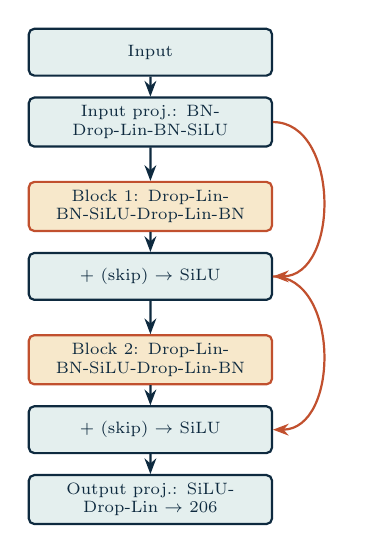
\begin{tikzpicture}[node distance=3mm, scale=0.85, transform shape,
          layer/.append style={text width=34mm},
          layerhi/.append style={text width=34mm}]
        \node[layer] (in) {Input};
        \node[layer, below=of in] (proj) {Input proj.: BN-Drop-Lin-BN-SiLU};
        \node[layerhi, below=5mm of proj] (b1) {Block 1: Drop-Lin-BN-SiLU-Drop-Lin-BN};
        \node[layer, below=of b1] (add1) {$+$ (skip) $\to$ SiLU};
        \node[layerhi, below=5mm of add1] (b2) {Block 2: Drop-Lin-BN-SiLU-Drop-Lin-BN};
        \node[layer, below=of b2] (add2) {$+$ (skip) $\to$ SiLU};
        \node[layer, below=of add2] (out) {Output proj.: SiLU-Drop-Lin $\to$ 206};

        \draw[flowarr] (in) -- (proj);
        \draw[flowarr] (proj) -- (b1);
        \draw[flowarr] (b1) -- (add1);
        \draw[flowarr] (add1) -- (b2);
        \draw[flowarr] (b2) -- (add2);
        \draw[flowarr] (add2) -- (out);

        \draw[flowarr, accent2, thick] (proj.east) .. controls +(10mm,0) and +(10mm,0) .. (add1.east);
        \draw[flowarr, accent2, thick] (add1.east) .. controls +(10mm,0) and +(10mm,0) .. (add2.east);
      \end{tikzpicture}
    \end{column}
    \begin{column}{0.58\textwidth}
      \begin{itemize}
        \item The curved orange arrows are the \textbf{residual (skip) connections}: the block's input is added to its output
        \item Eases gradient flow, stabilises deeper networks
        \item 2 residual blocks, \texttt{hidden\_dim = 512}, dropout 0.2
        \item Consumes \textbf{RankGauss + PCA} features: the transformed features \emph{plus} 50 + 15 PCA components ($\approx$950 inputs)
      \end{itemize}
    \end{column}
  \end{columns}
\end{frame}

% ---------------------------------------------------------------
% FT-TRANSFORMER
% ---------------------------------------------------------------
\begin{frame}{FT-Transformer -- How It Works}
  \begin{columns}[T]
    \begin{column}{0.58\textwidth}
      \centering
      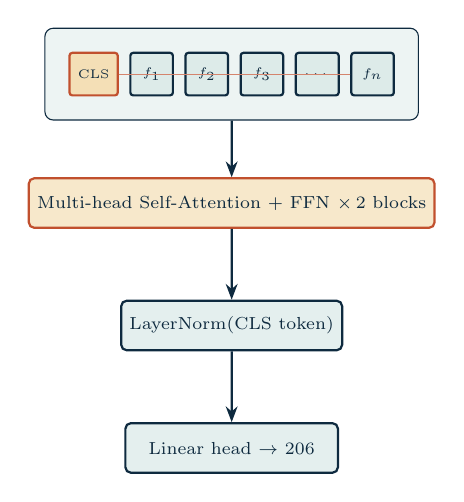
\begin{tikzpicture}[scale=0.9, transform shape]
          % token row
          \node[clstok] (cls) at (0,0) {CLS};
          \node[tok, right=1.5mm of cls] (t1) {$f_1$};
          \node[tok, right=1.5mm of t1] (t2) {$f_2$};
          \node[tok, right=1.5mm of t2] (t3) {$f_3$};
          \node[tok, right=1.5mm of t3] (t4) {$\cdots$};
          \node[tok, right=1.5mm of t4] (t5) {$f_n$};

          % attention links between tokens
          \foreach \a in {cls,t1,t2,t3,t5} {
            \foreach \b in {cls,t1,t2,t3,t5} {
              \draw[attn] (\a) -- (\b);
            }
          }

          % container box around the tokens
          \begin{scope}[on background layer]
            \node[
              draw=primary,
              fill=secondary!8,
              rounded corners=3pt,
              inner sep=3mm,
              fit=(cls) (t5)
            ] (tokens_box) {};
          \end{scope}

          % encoder, normalisation and head
          \node[layerhi, below=8mm of tokens_box, minimum width=55mm] (enc) {Multi-head Self-Attention + FFN $\times\,2$ blocks};
          \node[layer, below=of enc, minimum width=30mm] (ln) {LayerNorm(CLS token)};
          \node[layer, below=of ln, minimum width=30mm] (head) {Linear head $\to$ 206};

          \draw[flowarr] (tokens_box.south) -- (enc.north);
          \draw[flowarr] (enc) -- (ln);
          \draw[flowarr] (ln) -- (head);
        \end{tikzpicture}
    \end{column}
    \begin{column}{0.42\textwidth}
      \begin{itemize}
        \item Each scalar feature $\to$ its own \textbf{token} ($\approx$890 tokens/row incl.\ CLS)
        \item A learnable \textbf{[CLS]} token is prepended
        \item \textbf{Self-attention} (thin lines) connects every token to every other
        \item The CLS output summarises the row $\to$ classification head
        \item $O(L^2)$ cost $\Rightarrow$ smaller batch size (64)
        \item Consumes \textbf{raw RankGauss} features (no PCA)
        \item Simplified variant of Gorishniy et al.\ (post-LayerNorm, GELU, no ReGLU)
      \end{itemize}
    \end{column}
  \end{columns}
\end{frame}

% ---------------------------------------------------------------
% CATBOOST
% ---------------------------------------------------------------
\begin{frame}{CatBoost -- How It Works}
  \begin{columns}[T]
    \begin{column}{0.58\textwidth}
      \centering
      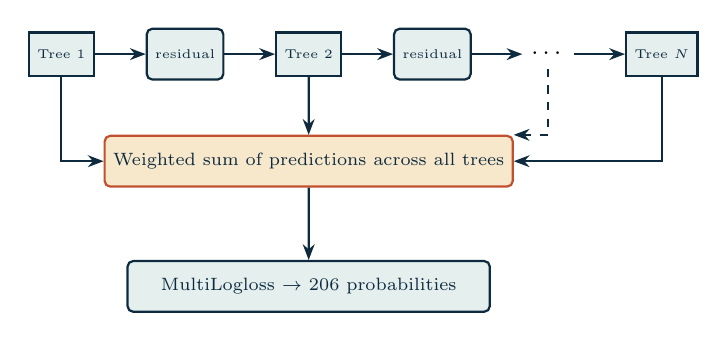
\begin{tikzpicture}[scale=0.92, transform shape]
        \node[tree] (t1) at (0,0) {Tree 1};
        \node[layer, right=7mm of t1, font=\tiny] (r1) {residual};
        \node[tree, right=7mm of r1] (t2) {Tree 2};
        \node[layer, right=7mm of t2, font=\tiny] (r2) {residual};
        \node[right=7mm of r2] (dots) {$\cdots$};
        \node[tree, right=7mm of dots] (t3) {Tree $N$};

        \draw[flowarr] (t1) -- (r1);
        \draw[flowarr] (r1) -- (t2);
        \draw[flowarr] (t2) -- (r2);
        \draw[flowarr] (r2) -- (dots);
        \draw[flowarr] (dots) -- (t3);
        \node[layerhi, below=8mm of t2, minimum width=55mm] (sum) {Weighted sum of predictions across all trees};
        \node[layer, below=of sum, minimum width=50mm] (out) {MultiLogloss $\to$ 206 probabilities};
        \draw[flowarr] (t1.south) |- (sum.west);
        \draw[flowarr] (t2.south) -- (sum.north);
        \draw[flowarr] (t3.south) |- (sum.east);
        \draw[flowarr, dashed] (dots.south) |- (sum.north east);
        \draw[flowarr] (sum) -- (out);
      \end{tikzpicture}
    \end{column}
    \begin{column}{0.42\textwidth}
      \begin{itemize}
        \item \textbf{Gradient boosting}: each tree corrects the residual error of the previous ones
        \item A single multi-output \texttt{MultiLogloss} fit, not 206 separate fits
        \item Splits stay aligned to the original features $\to$ trained on \textbf{raw RankGauss} (no PCA)
        \item Fixed 250 iterations (no early stopping), one fit per fold, no seed bagging
        \item Targets constant within a fold are excluded from the fit and filled with the observed constant
      \end{itemize}
    \end{column}
  \end{columns}
\end{frame}

\section{Training}

% ---------------------------------------------------------------
% METRIC, LOSS, TRAINING ROUTINE
% ---------------------------------------------------------------
\begin{frame}{Metric, Loss Variants and Training Routine}
  \begin{columns}[T]
    \begin{column}{0.5\textwidth}
      \textbf{Evaluation metric}
      \[
        \mathcal{L} = -\frac{1}{N \cdot 206}\sum_{i=1}^{N}\sum_{j=1}^{206}
        \Big[y_{ij}\log \hat y_{ij} + (1-y_{ij})\log(1-\hat y_{ij})\Big]
      \]
      predictions clipped to $[\epsilon, 1-\epsilon]$, with $\epsilon = 10^{-15}$, computed in float64.
      \\
      \vspace{4mm}
      \textbf{Optional variants (training loss only)}
      \begin{itemize}
        \item \textbf{Focal loss:} down-weights easy examples (off by default)
        \item \textbf{Label smoothing} (0.001): $y(1-\epsilon) + 0.5\epsilon$
        \item Model selection \textbf{always} uses the plain, non-smoothed log loss
      \end{itemize}
    \end{column}
    \begin{column}{0.5\textwidth}
      \begin{itemize}
        \item \textbf{AMP} (\texttt{torch.amp.GradScaler}) for speed and stability
        \item \textbf{Early stopping} (patience = 8 epochs) and \textbf{ReduceLROnPlateau}, both on the inner split
        \item Seeds set \emph{before} the model is built: initial weights depend on the seed
        \item \textbf{In-RAM checkpointing}: best \texttt{state\_dict} cloned to CPU, written to disk once at the end
        \item Explicit \texttt{torch.cuda.empty\_cache()} so sibling workers reclaim VRAM
      \end{itemize}
      \begin{alertblock}{Why it matters}
        Avoids dozens of slow disk writes per fold and prevents GPU memory creep across 30 jobs.
      \end{alertblock}
    \end{column}
  \end{columns}
\end{frame}

% ---------------------------------------------------------------
% VALIDATION PROTOCOL
% ---------------------------------------------------------------
\begin{frame}{Validation Protocol}
  \begin{columns}[T]
    \begin{column}{0.5\textwidth}
      \begin{block}{Outer loop: 5-fold OOF}
        \texttt{MultilabelStratifiedKFold}, seed 42. Each fold's validation part yields the out-of-fold predictions and is scored \textbf{once}, after training.
      \end{block}
      \begin{block}{Inner split: model selection}
        10\% of each training fold (stratified) drives early stopping, LR scheduling and best-epoch choice of the neural networks. CatBoost uses fixed iterations.
      \end{block}
    \end{column}
    \begin{column}{0.5\textwidth}
      \begin{block}{Blend: nested CV}
        Weights are fitted on $k-1$ folds' OOF predictions and scored on the held-out fold.
      \end{block}
      \begin{alertblock}{Known limitation}
        The data has no drug identifier, so the CV cannot be grouped by compound: the same compound may appear in training and validation. Scores can be optimistic compared with the leaderboard.
      \end{alertblock}
    \end{column}
  \end{columns}
\end{frame}

% ---------------------------------------------------------------
% PREPROCESSING
% ---------------------------------------------------------------
\begin{frame}{Two Preprocessing Pipelines}
  \begin{columns}[T]
    \begin{column}{0.5\textwidth}
      \begin{block}{PCA variant (ResNet)}
        VarianceThreshold $\to$ RankGauss (\texttt{QuantileTransformer}) $\to$ PCA(50) on \texttt{g-}, PCA(15) on \texttt{c-} $\to$ \textbf{concatenate} transformed features, PCA components and raw dummies ($\approx$950 columns)
      \end{block}
    \end{column}
    \begin{column}{0.5\textwidth}
      \begin{block}{Raw variant (FT-Transformer, CatBoost)}
        VarianceThreshold $\to$ RankGauss, \textbf{no PCA} -- keeps one token/split per original feature ($\approx$890 columns)
      \end{block}
    \end{column}
  \end{columns}
  \vspace{2mm}
  \small Both fitted \textbf{per fold} on the training split only and cached to disk as \texttt{.joblib}. The raw pipeline fitted for the transformer is reused by CatBoost within the same run; stale caches are cleared at the start of each run.
\end{frame}

\section{Cross-Validation \& Ensembling}

% ---------------------------------------------------------------
% NN CV AT SCALE
% ---------------------------------------------------------------
\begin{frame}[fragile]{NN Cross-Validation at Scale}
  \begin{columns}[T]
    \begin{column}{0.55\textwidth}
      \begin{itemize}
        \item $2$ networks $\times$ $3$ seeds $\times$ $5$ folds $=$ \textbf{30 jobs}
        \item \texttt{joblib} + \texttt{loky} backend, GPUs assigned \textbf{round-robin}
        \item 2 GPUs $\times$ 2 jobs/GPU $=$ \textbf{4 parallel workers}
        \item Predictions averaged over the 3 seeds per (fold, model)
        \item Wall-clock: NN CV 96.3 min, CatBoost CV 29.7 min, inference 0.5 min
      \end{itemize}
    \end{column}
    \begin{column}{0.45\textwidth}
      \begin{lstlisting}
NN_JOBS_PER_GPU = 2
N_JOBS_NN = N_GPUS * NN_JOBS_PER_GPU

Parallel(n_jobs=N_JOBS_NN,
         backend="loky")(
  delayed(_train_nn_job)(...)
  for job in jobs
)
      \end{lstlisting}
    \end{column}
  \end{columns}
\end{frame}

% ---------------------------------------------------------------
% BLENDING METHODOLOGY
% ---------------------------------------------------------------
\begin{frame}{Ensemble Blending: Methodology}
  \begin{columns}[T]
    \begin{column}{0.5\textwidth}
      \textbf{Weight search}
      \begin{itemize}
        \item Softmax-reparameterised weights on the simplex
        \item \textbf{Nelder--Mead}, not SLSQP: avoids a zero finite-difference gradient stalling the optimiser at $x_0$
      \end{itemize}
    \end{column}
    \begin{column}{0.5\textwidth}
      \textbf{Nested CV}
      \begin{itemize}
        \item Weights fit on $k-1$ folds, scored on the held-out fold
        \item Prevents an over-optimistic blend score
        \item Final weights = mean across folds
      \end{itemize}
    \end{column}
  \end{columns}
  \begin{exampleblock}{Two scores reported}
    \emph{naive} OOF blend score (same data used to fit the weights) vs.\ \emph{honest} nested-CV score
  \end{exampleblock}
\end{frame}

\section{Results}

% ---------------------------------------------------------------
% RESULTS: FOLD BY FOLD
% ---------------------------------------------------------------
\begin{frame}{Results -- Fold-by-Fold Validation Loss}
  \centering
  \begin{tabular}{@{}cccc@{}}
    \toprule
    \textbf{Fold} & \textbf{ResNet} & \textbf{FT-Transformer} & \textbf{CatBoost} \\
    \midrule
    0 & 0.01686 & 0.01693 & 0.01707 \\
    1 & 0.01705 & 0.01710 & 0.01709$^{*}$ \\
    2 & 0.01652 & 0.01656 & 0.01676 \\
    3 & 0.01679 & 0.01688 & 0.01704$^{*}$ \\
    4 & 0.01700 & 0.01705 & 0.01704 \\
    \midrule
    \textbf{Mean} & 0.01684 & 0.01690 & 0.01700 \\
    \bottomrule
  \end{tabular}
  \vspace{2mm}

  \small $^{*}$ 1 constant target in the training fold, excluded from the CatBoost fit and filled with the observed constant.
  \vspace{2mm}

  \small Network values are the \emph{mean of the per-seed losses}; CatBoost is trained once per fold. The OOF scores on the next slide use \emph{seed-averaged predictions}, which lowers the loss by about 0.0005 (bagging gain). ResNet is the best network in every fold.
\end{frame}

% ---------------------------------------------------------------
% RESULTS: OOF SUMMARY + CHART
% ---------------------------------------------------------------
\begin{frame}{Results -- Out-of-Fold Summary}
  \begin{columns}[T]
    \begin{column}{0.48\textwidth}
      \centering
      \begin{tabular}{@{}lc@{}}
        \toprule
        \textbf{Model} & \textbf{OOF log loss} \\
        \midrule
        ResNet & \textbf{0.01632} \\
        FT-Transformer & 0.01643 \\
        CatBoost & 0.01700 \\
        \midrule
        Ensemble (nested) & \textbf{0.01606} \\
        \bottomrule
      \end{tabular}
      \vspace{3mm}

      \small\textbf{Timing:} NN CV 96.3 min \textbar\ CatBoost CV 29.7 min \textbar\ total 128.6 min
    \end{column}
    \begin{column}{0.52\textwidth}
      \centering
      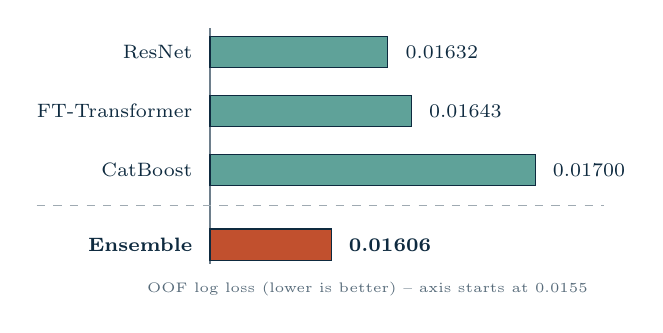
\begin{tikzpicture}[scale=1, every node/.style={font=\scriptsize}]
        % baseline axis; bar length = (loss - 0.0155) * 27.5 mm per 0.001
        \draw[primary!60] (0,3mm) -- (0,-27mm);
        \foreach \lbl/\w/\y/\col/\val in {
          ResNet/22.6mm/0mm/secondary!70/0.01632,
          {FT-Transformer}/25.6mm/-7.5mm/secondary!70/0.01643,
          CatBoost/41.3mm/-15mm/secondary!70/0.01700
        } {
          \node[anchor=east, text=primary] at (-1mm,\y) {\lbl};
          \draw[fill=\col, draw=primary] (0,\y-2mm) rectangle (\w,\y+2mm);
          \node[anchor=west, text=primary] at (\w+1mm,\y) {\val};
        }
        \draw[primary!40, dashed] (-22mm,-19.5mm) -- (50mm,-19.5mm);
        \node[anchor=east, text=primary, font=\scriptsize\bfseries] at (-1mm,-24.5mm) {Ensemble};
        \draw[fill=accent2, draw=primary] (0,-26.5mm) rectangle (15.4mm,-22.5mm);
        \node[anchor=west, text=primary, font=\scriptsize\bfseries] at (16.4mm,-24.5mm) {0.01606};
        \node[anchor=north, text=primary!70, font=\tiny] at (20mm,-28mm) {OOF log loss (lower is better) -- axis starts at 0.0155};
      \end{tikzpicture}
    \end{column}
  \end{columns}
\end{frame}

% ---------------------------------------------------------------
% RESULTS: NESTED BLEND
% ---------------------------------------------------------------
\begin{frame}{Results -- Ensemble Blend (Nested CV)}
  \centering
  {\large\bfseries Score and weights per held-out fold}\\[1mm]
  \begin{tabular}{@{}ccccc@{}}
    \toprule
    \textbf{Fold} & \textbf{Score} & $w_{\text{resnet}}$ & $w_{\text{ft}}$ & $w_{\text{cb}}$ \\
    \midrule
    0 & 0.01603 & 0.447 & 0.374 & 0.179 \\
    1 & 0.01618 & 0.460 & 0.369 & 0.170 \\
    2 & 0.01570 & 0.437 & 0.373 & 0.190 \\
    3 & 0.01617 & 0.428 & 0.389 & 0.183 \\
    4 & 0.01622 & 0.465 & 0.370 & 0.166 \\
    \bottomrule
  \end{tabular}

  \vspace{0.4cm}

  \begin{columns}[T]
    \begin{column}{0.48\textwidth}
      \begin{block}{Final weights (mean across folds)}
        \small
        ResNet 44.7\% \textbar\ FT-Transformer 37.5\% \textbar\ CatBoost 17.8\%
      \end{block}
    \end{column}
    \begin{column}{0.48\textwidth}
      \begin{exampleblock}{Honest nested-blend score}
        $0.01606 \pm 0.00019$
      \end{exampleblock}
    \end{column}
  \end{columns}

  \vspace{1mm}
  \small Naive OOF blend (0.01606) equals the nested score. With only three weights this is expected; it does not rule out leakage from the CV design (no grouping by compound).
\end{frame}

\begin{frame}{Ablation -- Is an Extra Network Worth It?}
  \centering
  \begin{tabular}{@{}lccc@{}}
    \toprule
    \textbf{Base: ResNet + FT + CatBoost} & \textbf{Extra OOF} & \textbf{Ensemble (nested)} & \textbf{Extra weight} \\
    \midrule
    + MLP (PCA features) & 0.01649 & 0.01604 & 1.5\% \\
    + 1D-CNN (PCA features) & 0.01661 & 0.01605 & 8.2\% \\
    + 1D-CNN (raw features) & 0.01661 & 0.01606 & 7.0\% \\
    \textbf{no extra network (final)} & -- & \textbf{0.01606} & -- \\
    \bottomrule
  \end{tabular}
  \vspace{4mm}

  \begin{columns}[T]
    \begin{column}{0.48\textwidth}
      \begin{block}{Reading}
        \small All four ensembles score 0.01604--0.01606: the differences ($\le 2\cdot10^{-5}$) are below the fold standard deviation (0.00018) and the run-to-run GPU noise ($\approx 10^{-5}$).
      \end{block}
    \end{column}
    \begin{column}{0.48\textwidth}
      \begin{exampleblock}{Decision}
        \small The extra network earns weight but no measurable gain, even with raw features. The simpler 3-model blend is kept: fewer components to train, explain and maintain.
      \end{exampleblock}
    \end{column}
  \end{columns}
\end{frame}

\section{Conclusions}

% ---------------------------------------------------------------
% CONCLUSIONS
% ---------------------------------------------------------------
\begin{frame}{Conclusions, Limitations and Future Work}
  \small
  \begin{columns}[T]
    \begin{column}{0.5\textwidth}
      \textbf{Findings}
      \begin{itemize}
        \item Ensemble 0.01606 vs.\ best single model (ResNet) 0.01632: $\approx$1.6\% better
        \item ResNet and FT-Transformer carry $\approx$82\% of the weight; CatBoost, weakest alone, gets 18\%
        \item An extra network (MLP or 1D-CNN, on PCA or raw features) does not improve the blend
      \end{itemize}
      \textbf{Future work}
      \begin{itemize}
        \item Group the CV by compound; measure the leaderboard score
        \item Ablations: PCA vs.\ raw for the ResNet, error correlation between models
      \end{itemize}
    \end{column}
    \begin{column}{0.5\textwidth}
      \textbf{Limitations}
      \begin{itemize}
        \item No compound identifier: possible leakage across folds, optimistic scores
        \item The inner split removes 10\% of the training data; an earlier protocol that selected epochs on the OOF fold gave 0.01595, so about 0.0001 of that gap was optimism
        \item GPU non-determinism: repeated runs differ by $\approx 10^{-5}$; wall-clock time varied by about 20\% across runs
        \item Why CatBoost earns weight (diverse errors) was not measured
      \end{itemize}
    \end{column}
  \end{columns}
\end{frame}

% ---------------------------------------------------------------
% REFERENCES
% ---------------------------------------------------------------
\begin{frame}{References}
  \scriptsize
  \begin{itemize}
    \item Kaggle, \emph{Mechanisms of Action (MoA) Prediction}, 2020. \url{https://www.kaggle.com/competitions/lish-moa}
    \item Gorishniy et al., \emph{Revisiting Deep Learning Models for Tabular Data}, NeurIPS 2021 (FT-Transformer).
    \item Prokhorenkova et al., \emph{CatBoost: unbiased boosting with categorical features}, NeurIPS 2018.
    \item Sechidis, Tsoumakas, Vlahavas, \emph{On the Stratification of Multi-Label Data}, ECML PKDD 2011.
    \item Bradberry, \emph{iterative-stratification} (Python package). \url{https://github.com/trent-b/iterative-stratification}
    \item Paszke et al., \emph{PyTorch}, NeurIPS 2019; Pedregosa et al., \emph{Scikit-learn}, JMLR 12, 2011.
    \item Loshchilov, Hutter, \emph{Decoupled Weight Decay Regularization} (AdamW), ICLR 2019.
    \item Micikevicius et al., \emph{Mixed Precision Training}, ICLR 2018.
    \item Lin et al., \emph{Focal Loss for Dense Object Detection}, ICCV 2017; Szegedy et al., \emph{Rethinking the Inception Architecture} (label smoothing), CVPR 2016.
    \item Nelder, Mead, \emph{A simplex method for function minimization}, The Computer Journal 7(4), 1965.
  \end{itemize}
\end{frame}

\end{document}
